\graphicspath{{results/fig/}}

\chapter{Results}
\label{chap:results}
An incremental approach to testing was done for this project. Each software component was tested individually. This section will report on the results of the incremental testing as well as the results of the entire system. As a sanity check, the results will also be compared to the results in \cite{fluxNoiseSquidsStevenAnton}. Lastly the entire system will be used to calculate the mean square flux noise figure of an actual SQUID design. Low frequency flux noise is typically reported in terms of a power spectral density. To relate the power spectral density to the mean square flux noise one can simply apply equation \ref{eq:PSDtoMSFN}.
\begin{equation}
    \langle \Phi^2 \rangle = \int_{f_1}^{f_2}S_\Phi (f) df
    \label{eq:PSDtoMSFN}
\end{equation} 
The limits of the integral are still the subject of debate \cite{fluxNoiseSquidsStevenAnton}. For the purposes of this analysis, the example of \cite{fluxNoiseSquidsStevenAnton} will be followed and $f_1$ is choosen to be $10^{-2}$. The value of $f_2$ is not known, and will therefore be arbitrarily chosen to be $10^6$. The value for the MSFN figure will then not be exact as the bandwidth of the noise process is not known. This analysis will hope to show trends between measured flux noise power spectral densities and the MSFN figure produced by the noise extraction module.
\section{The noise extraction module}
The accuracy of this module is tested by comparing its output to a numerical solution for the given geometry. This module is tested without mesh optimisation. It is tested before the mesh optimisation module because the test setup for the mesh optimisation module requires the use of the noise extraction module.
\subsection{Test setup}
The aim of this project is not to verify the numerical framework proposed in \cite{fluxNoiseSquidsStevenAnton}. The testing should reflect this. As such the test setup is designed to verify the functionality of the implementation allowing the geometry of such a setup to not be limited by realistic designs for SQUID washers. Equation \ref{eq:MSFNfinal} describes the analytical solution for a thin wire loop. The assumption made in the derivation of this equation is that $R >> D$. The test is performed was a parameter sweep from $R = \si{8}{\mu m}$ and $D = \si{5}{\mu m}$ to $R = \si{45}{\mu m}$ and $D = \si{0.4}{\mu m}$ as shown figure \ref{fig:meshedTorus}. The parameter sweep was automated using a python script.

\begin{figure}[h]
    \centering
    \begin{subfigure}[b]{0.45\textwidth}
        \centering
        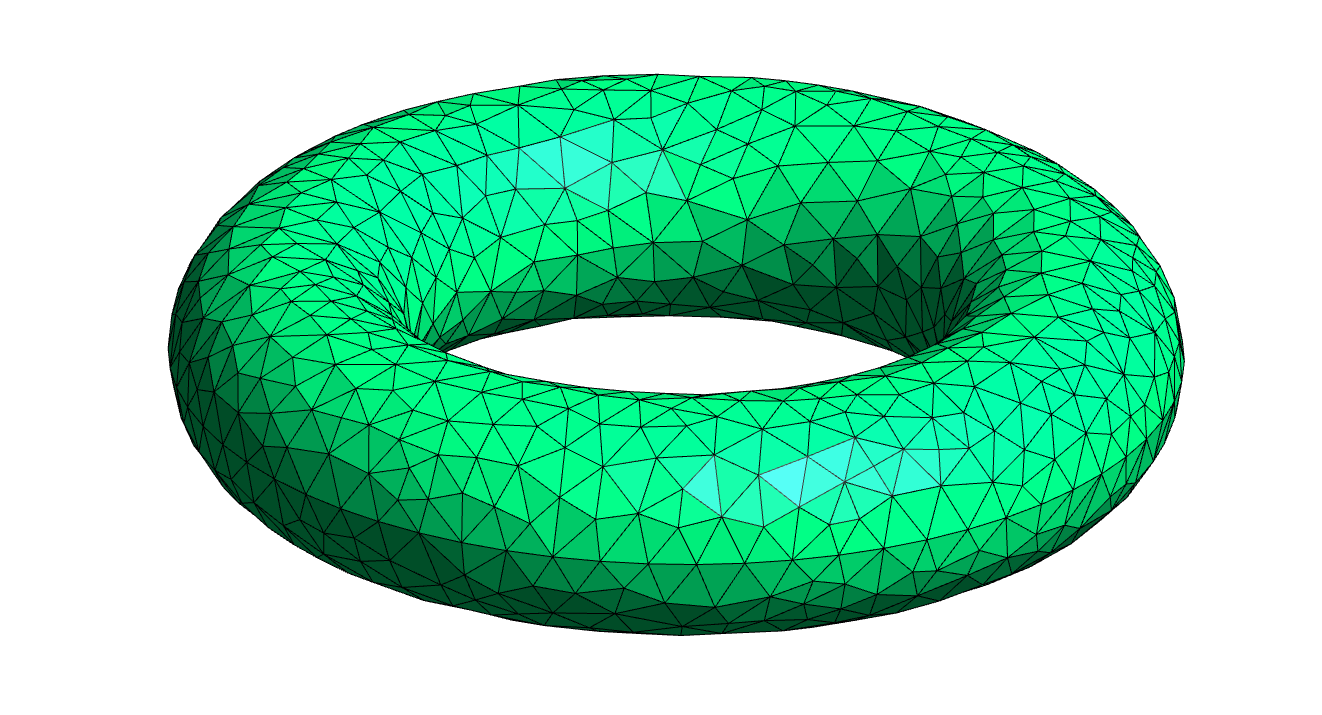
\includegraphics[width=0.5\textwidth]{torusThick}
        \caption{The meshed torus with the smallest loop radius and largest wire diameter}
    \end{subfigure}
    \hfill
    \begin{subfigure}[b]{0.45\textwidth}
        \centering
        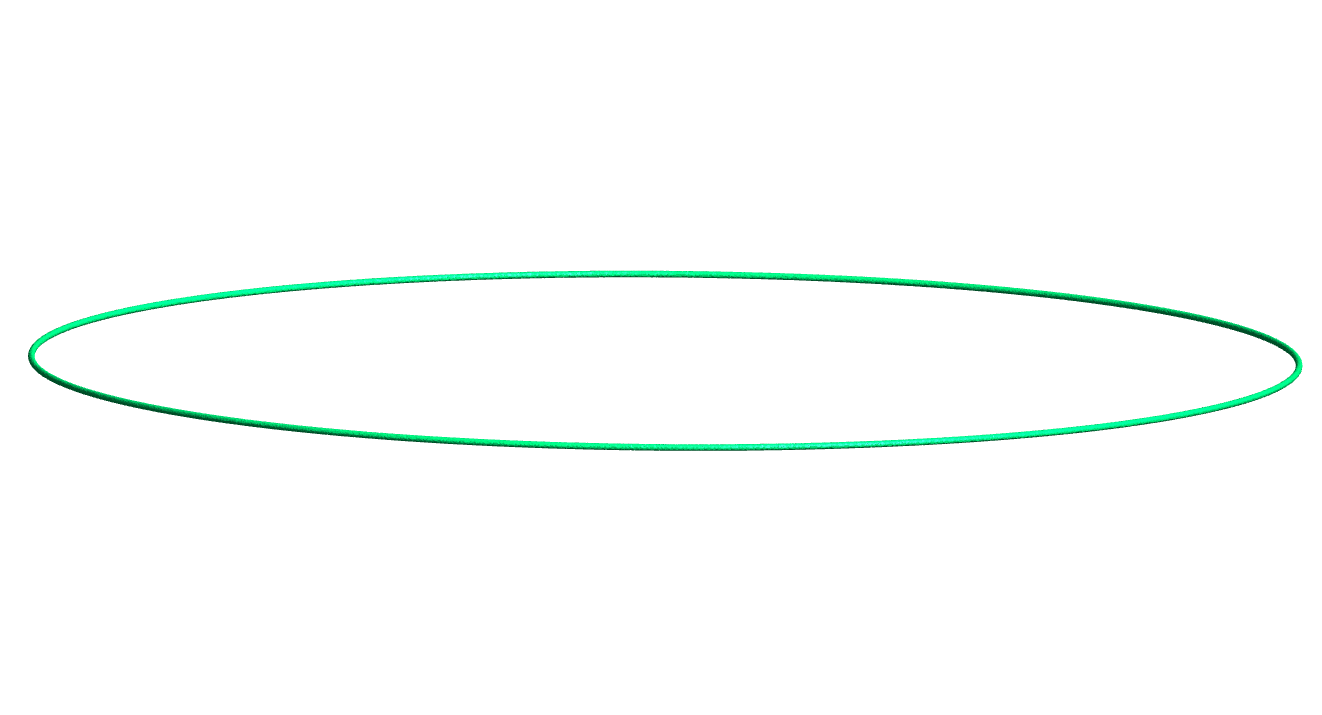
\includegraphics[width=0.5\textwidth]{torusThin}
        \caption{The meshed torus with the largest loop radius and smallest wire diameter}
    \end{subfigure}
    \caption{A figure showing the two extremes of the parameter sweep for a torus. The images show the surface mesh as generated by GMSH.}
    \label{fig:meshedTorus}
\end{figure}
\subsection{Results}

The results of the parameter sweep are summarized in figure \ref{fig:resTorus}.
\begin{figure}[H]
    \centering
    \begin{subfigure}[b]{0.48\textwidth}
        \centering
        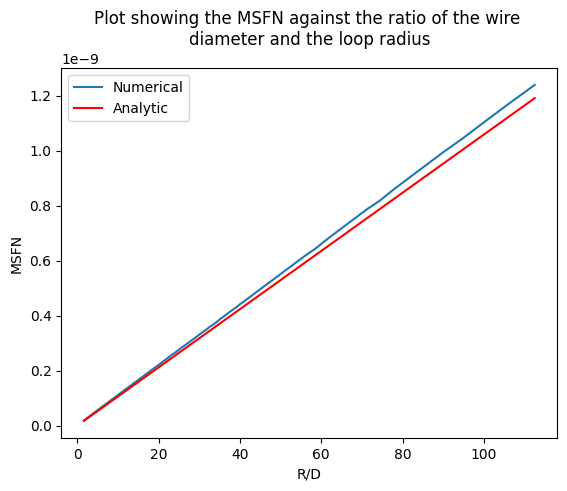
\includegraphics[width=\textwidth]{torusAVN}
        \caption{The analytical and numerical solutions for the parameter sweep}
        \label{fig:MSFNvRD}
    \end{subfigure}
    \hfill
    \begin{subfigure}[b]{0.48\textwidth}
        \centering
        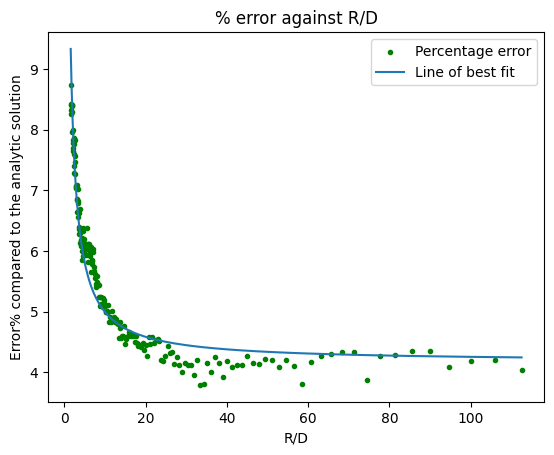
\includegraphics[width=\textwidth]{torusEVRD}
        \caption{The error plotted against the $R/D$}
        \label{fig:evRD}
    \end{subfigure}
    \caption{The figure shows both the MSFN ($\Phi_0^2 / Hz$) and the error compared to the analytic solution for the parameter sweep.}
    \label{fig:resTorus}
\end{figure}
From figure \ref{fig:resTorus} it is clear to see that the relative percentage error compared to the analytic solution decreases as the ration of the loop radius to diameter increases. This behaviour can be attributed to the assumption: $R >> D$. The decrease in error clearly demonstrates that the noise extraction module works for this particular setup. In figure \ref{fig:MSFNvRD} the analytical and numerical results increase linearly with an increase in $\frac{R}{D}$ as expected.

\section{The mesh optimisation module}
The geometry used to test the noise extraction module is not ideal for testing the mesh optimisation algorithm. To understand why this is the case, one must consider the assumption made to derive the analytic solution. By assuming that $R >> D$ you can approximate the ring as an infinitely long wire. By extension this assumes that the magnetic flux density and current density is uniform across the surface of the ring. The testing of the noise extraction module showed that the approximation is quite good. As a consequence, the mesh optimisation algorithm does not do much because the consistent current distribution leads to the mesh being over refined everywhere or not refined at all.
\subsection{Test setup}
To test this module a thin film circular ring of loop radius $R$ and track width $W$ is used. Essentially 3 questions must be answered. How many optimisation iterations is required, how much faster the problem is solved with the optimized mesh and if the subsequent extra executions of GMSH and TetraHenry needed to optimize the mesh is worth the trouble. \par
The test setup once again consists of a parameter sweep of $R$ and $W$ over the ranges $10 \mu m \le R \le 15 \mu m $ and $  3 \mu m \le W \le7\mu m$. The two extremes of the parameter sweep is shown in figure \ref{fig:testloop}. Simulations are run at 50 linearly spaced points in these intervals. For each simulation iteration, 4 mesh optimisation iterations are run. The initial characteristic length is determined by GMSH. The average mesh element count was $1500$ elements. Testing is once again completely automated with python. At each iteration the script records a number of statistics. The script records the execution times of TetraHenry and GMSH. It keeps track of both the simulation iteration and the mesh optimisation iteration. The results are written to a CSV file to be analysed with the \textit{"pandas"} python package. 
\begin{figure}[H]
    \centering
    \begin{subfigure}[b]{0.48\textwidth}
        \centering
        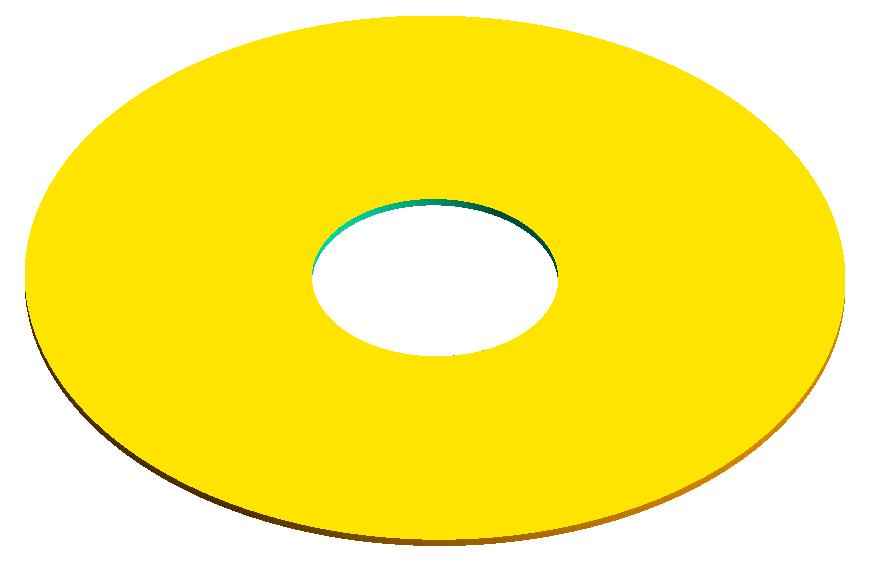
\includegraphics[width=\textwidth]{thickloop}
        \caption{The geometry of the test setup for the first iteration}
        \label{fig:thickloop}
    \end{subfigure}
    \hfill
    \begin{subfigure}[b]{0.48\textwidth}
        \centering
        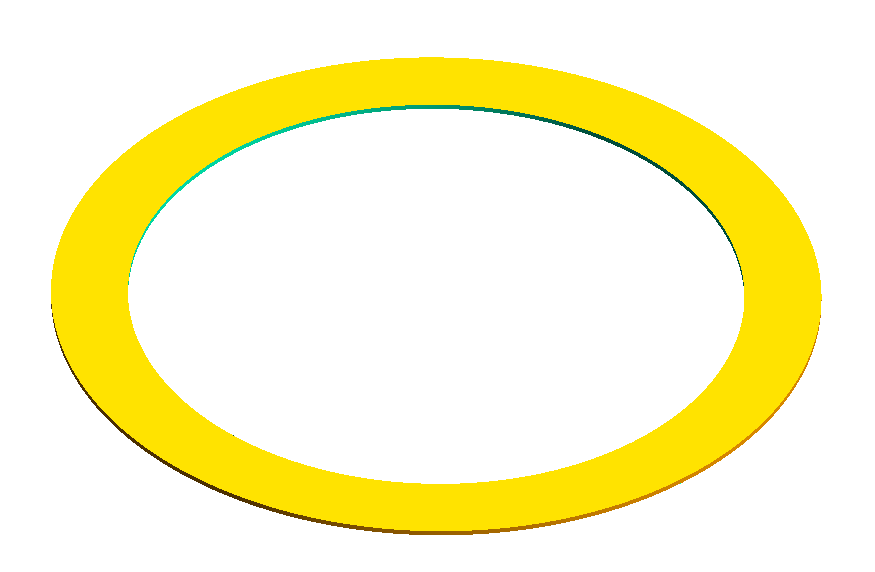
\includegraphics[width=\textwidth]{thinloop}
        \caption{The geometry of the test setup for the last iteration}
        \label{fig:thinloop}
    \end{subfigure}
    \caption{The figure shows the 2 extremes in the parameter sweep for the thin film circular loop experiment. The track thickness is set to $0.1 \mu m$}
    \label{fig:testloop}
\end{figure}
To assess the effectivity of the mesh optimisation algorithm it is necessary to make a baseline measurement. The baseline is set by forcing a minimum characteristic length in the optimized mesh and comparing the result to an unoptimized mesh with characteristic length equal to the minimum characteristic length in the optimized mesh.

\subsection{Results}

To determine the number of optimisation steps necessary for convergence, the average relative error between the mean square flux noise figure calculated at each optimisation iteration and the value obtained after the $4_{th}$ optimisation iteration is calculated. The result is summarized in table \ref{tab:relerr}.


\begin{table}[H]
    \centering
    \begin{tabular}{lll}
    \hline
    Iteration number & Relative percentage error & Change in relative error \\ \hline
    0                & 1.520356                  & N/A                      \\
    1                & 0.47945                   & 1.040906                 \\
    2                & 0.028596                  & 0.450854                 \\
    3                & 0.001191                  & 0.027405                 \\
    4                & 0.000065                  & 0.001126                 \\ \hline         
    \end{tabular}
    \caption{Table of relative errors for each mesh optimisation cycle}
    \label{tab:relerr}
\end{table}

Table \ref{tab:relerr} gives some indication that after 4 iterations the solution becomes relatively stable. If we accept the 4 mesh optimisation iteration as being the correct result we can normalise the relative error and plot it against the normalised, cumulative time GMSH and TetraHenry took after each iteration. Figure \ref{fig:errvtime} shows this relationship.

\begin{figure}[H]
    \centering
    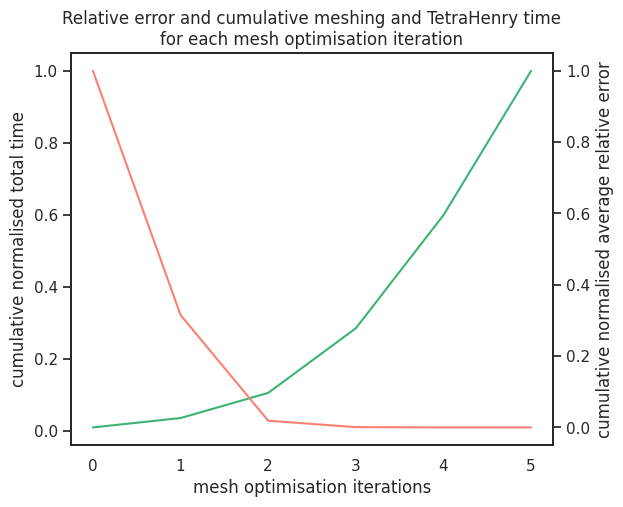
\includegraphics[width=0.5\linewidth]{errvtime}
    \caption{The figure shows the relative normalised error and the cumulative total time that GMSH and TetraHenry took at each optimisation step. The green line is the total time and the red line is the error.}
    \label{fig:errvtime}
\end{figure}

The optimal number of mesh iterations steps to minimize the time taken, and the error is between 1 and 2 iterations. The choice ultimately comes down to how accurate the user would like the solution to be. To compare the optimized mesh performance to the baseline, 2 will be selected as the optimal number of iterations. \par

\textcolor{red}{I need Dr Jackman to run more simulations for me. I have already sent him the files}

\section{Comparison with the results of S.M. Anton \textit{et al.}}
\subsection{Test Setup}
To verify the implementation of the numerical framework, a comparison with the results in \cite{fluxNoiseSquidsStevenAnton} is made. The same test will run for the exact same geometry. The setup chosen for this project consists of a square washer with a fixed square hole with a width of $10 \mu m$. The line width is then swept from $0.5 \mu m$ to $10 \mu m$. Figure \ref{fig:sqwasher} shows the geometry in the test setup. The film thickness is $150 \mu m$ and the penetration depth is identical to that used in \cite{fluxNoiseSquidsStevenAnton} and is set to $90 nm$. The implementation used in \cite{fluxNoiseSquidsStevenAnton} can be found here \cite{msfnCode} 

\begin{figure}[H]
    \centering
    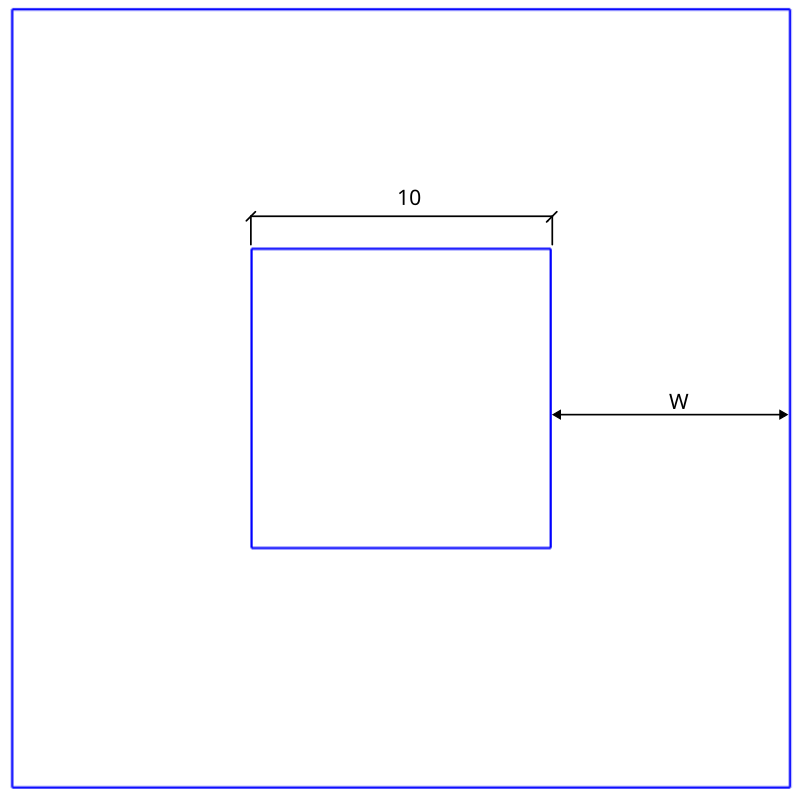
\includegraphics[width=0.3\linewidth]{sqwasher}
    \caption{The figure shows the geometry of the test washer in GMSH. All dimension are in $\mu m$}
    \label{fig:sqwasher}
\end{figure}

\subsection{Results}
Figure \ref{fig:steveComp} shows the results obtained by running the test setup. 
\begin{figure}[H]

    \centering
    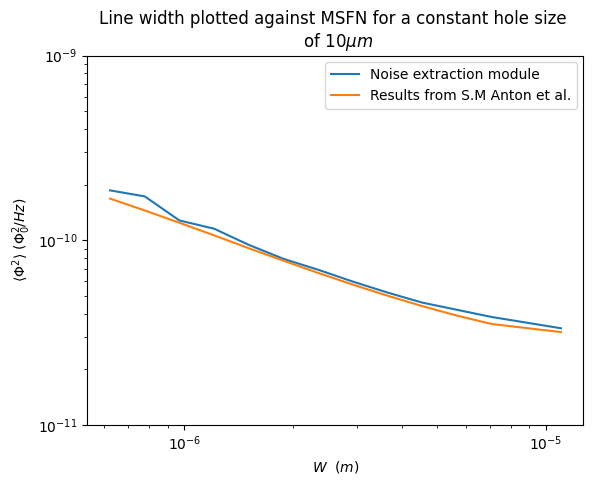
\includegraphics[width=0.4\linewidth]{steveComp}
    \caption{The plot shows the MSFN figure calculated by the noise extraction module as well as the figure calculated using \cite{msfnCode}}
    \label{fig:steveComp}
\end{figure}
From figure \ref{fig:steveComp} it is clear to see that the noise extraction module produces values in agreement with those obtained by S.M. Anton \textit{et al.} in \cite{fluxNoiseSquidsStevenAnton}. As shown in the previous section, the error decreases for an increase in optimisation iterations. One can therefore expect the noise extraction module to conform more closely to the results by S.M. Anton \textit{et al.} for a higher number of optimisation iterations. This could unfortunately not be tested due to memory limitations.

\section{Comparison with actual SQUID designs}
\subsection{Test setup}
Equation \ref{eq:PSDtoMSFN} can be used in conjunction with the parameters determined by F.C. Wellstood et al. \cite{FluxNoiseCol} to relate the output of the noise extraction module to practical measurements. The integration limits are determined by choosing $f1 = 10^{-1} Hz$ as this correspond to the lowest frequency measured in \cite{FluxNoiseCol}. The second limit is chosen such that the noise extraction module results approximately match the measured flux noise figures for 1 of the SQUID's. Both limits are then kept constant for varying SQUID geometries. \par
To simplify the structure of the SQUID washer the multi-layer design will be ignored. The SQUID will be modelled as a single layer washer. This is technically not accurate but the modelling of a multi-layer design is outside the scope of this project. The parameters are weak functions of the materials used and as such the choice of which material to use for the SQUID washer is not of importance. Figure \ref{fig:realCOMP} shows the various squid loop geometries analysed. 

\begin{figure}[H]
    \centering
    \begin{subfigure}[b]{0.4\textwidth}
        \centering
        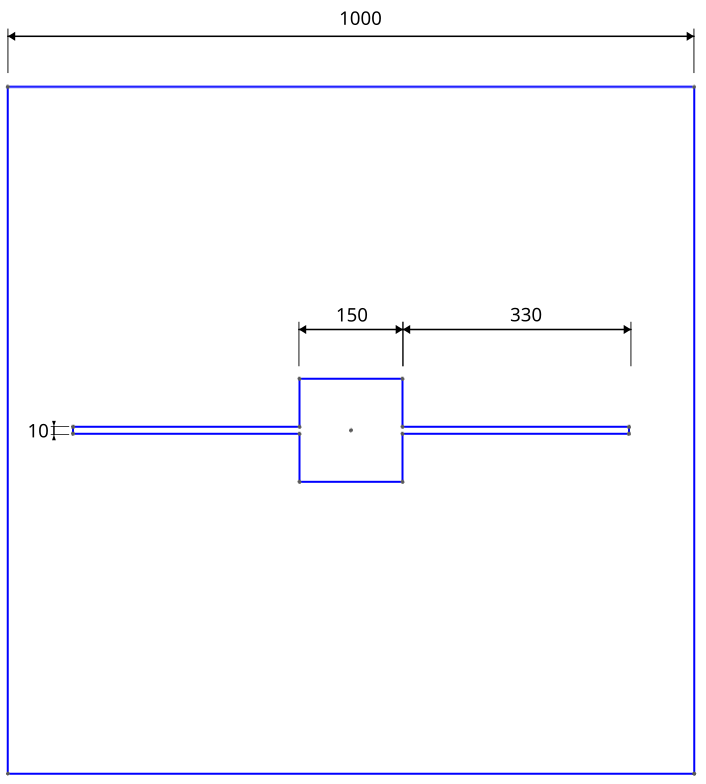
\includegraphics[width=\textwidth]{td1}
        \caption{The geometry used to analyse SQUID type D from \cite{FluxNoiseCol}.}
        \label{fig:type1D}
    \end{subfigure}
    \hfill
    \begin{subfigure}[b]{0.4\textwidth}
        \centering
        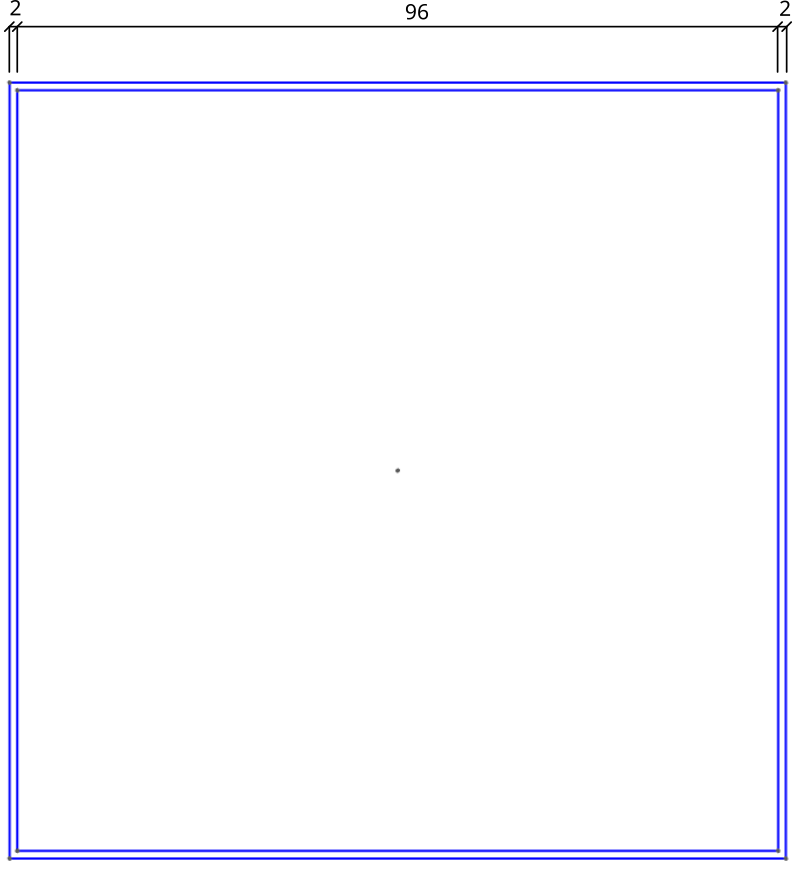
\includegraphics[width=\textwidth]{tf1}
        \caption{The geometry used to analyse SQUID type F from \cite{FluxNoiseCol}.}
        \label{fig:type1F}
    \end{subfigure}
    \caption{The two types of SQUID loops analysed with the noise extraction module. The type value corresponds to the naming scheme used in \cite{FluxNoiseCol}. All dimensions are in $\mu m$. All SQUID designs have the same film thickness of $0.2 \mu m$}
    \label{fig:realCOMP}
\end{figure}

\subsection{Results}
\textcolor{red}{I will do the analysis for 1 more SQUID}
Table \ref{tab:COMP} shows the predicted MSFN figure as well as the derived MSFN from the measured power spectral density. 
\begin{table}[H]
    \centering
    \begin{tabular}{lll}
    \hline
    SQUID Type & Predicted $\langle \Phi_0 ^2 \rangle$ & Measured $\langle \Phi_0 ^2 \rangle$ \\ \hline
    D          & $4.678e-10$                         & $5.644e-09$            \\
    F          & $2.708e-09$                         & $3.955e-08$            \\ \hline
    \end{tabular}
    \caption{The resulting MSFN figure predicted by the noise extraction module as well as the derived MSFN figure}
    \label{tab:COMP}
\end{table}

There is a large discrepancy in the predicted and derived figures. On average, the values vary by an order of magnitude. The noise extraction module predicts less noise than what is actually observed. The measurements where taken at very low temperatures (as low as $20 mk$) to limit the amount of critical current noise present in the system. This cannot completely eliminate the noise as that would require zero kelvin temperatures. This can account for a portion of the discrepancy but at the temperatures these measurements where taken it seems unlikely that it can be wholly attributed to critical current noise. Another likely source of error is the simplistic model for the SQUID washer. The arbitrary choice of integration limits is another potential source of error. \par 
Despite the large discrepancy the tool is useful as the trends across various geometries hold. This means that the tool can help designers choose loop geometries that improve on low frequency performance without being able to accurately predict the MSFN noise figure.